\documentclass[conference]{IEEEtran}
\IEEEoverridecommandlockouts

\usepackage{cite}
\usepackage{amsmath,amssymb,amsfonts}
\usepackage{graphicx}
\usepackage{textcomp}
\usepackage{xcolor}
\usepackage{booktabs}
\usepackage{url}
\usepackage{hyperref}
\hypersetup{colorlinks=true, linkcolor=blue, citecolor=blue, urlcolor=blue}

% Works both locally (figures one level up) and on Overleaf (figures at root)
\graphicspath{{./}{../figures/}}

\begin{document}

\title{Tip-of-the-Tongue Retrieval with Transformer-Based Reranking:\\
BM25, Cross-Encoder, and Bi-Encoder Compared}

\author{\IEEEauthorblockN{\.Ilayda Erg\"ur}
\IEEEauthorblockA{Department of Multimedia Informatics\\
Middle East Technical University\\
Ankara, Turkey\\
ilayda.ergur@metu.edu.tr}}

\maketitle

\begin{abstract}
This paper presents a complete, three-phase investigation of transformer-based reranking
for Tip-of-the-Tongue (ToT) retrieval on the TREC-ToT 2024 dataset.
Phase~1 characterised the corpus (3.18M Wikipedia documents) and revealed that all 142
evaluation queries share zero lexical overlap with their top BM25 candidate, establishing
that ToT is a purely semantic retrieval task.
Phase~2 tuned a BM25 baseline via a 20-run Weights \& Biases hyperparameter sweep
($k_1=1.2$, $b=0.75$; RR@10~=~0.0751) and evaluated a cross-encoder reranker
(\texttt{ms-marco-MiniLM-L-6-v2}; RR@10~=~0.0463), finding no statistically significant
improvement (Wilcoxon $p=0.1023$).
Phase~3 adds a bi-encoder reranker (\texttt{all-MiniLM-L6-v2}; RR@10~=~0.0534), selected
via a $2\times2$ model-and-depth sweep, together with Wilcoxon tests for all three pairwise
comparisons, t-SNE embedding projection, sentence-level cross-encoder attribution, and
systematic error analysis.
BM25 remains the strongest system in aggregate; neither neural model significantly
outperforms it at $\alpha=0.05$.
Subgroup analysis reveals that long queries ($>$121 words) cause substantial neural
degradation, and error analysis confirms that 82.4\% of all failures stem from the BM25
candidate pool not containing the relevant document---pointing to dense first-stage
retrieval as the critical unsolved bottleneck.
All code, experimental outputs, and Weights \& Biases sweep logs are publicly available.
\end{abstract}

\begin{IEEEkeywords}
tip-of-the-tongue retrieval, BM25, cross-encoder, bi-encoder, Wilcoxon test,
interpretability, t-SNE, TREC, sentence transformers, information retrieval
\end{IEEEkeywords}

% ══════════════════════════════════════════════════════════════════════════════
\section{Introduction}
% ══════════════════════════════════════════════════════════════════════════════

Retrieval of a forgotten entity from a long descriptive memory narrative---commonly called
Tip-of-the-Tongue (ToT) retrieval---is one of the most semantically demanding retrieval
scenarios studied in information retrieval~\cite{trec-tot}.
Unlike classical ad-hoc retrieval, where a user supplies a short keyword query that closely
mirrors the target document's vocabulary, a ToT query is a multi-sentence narrative of
100--400 words describing an entity whose name the user cannot recall.
Queries use subjective attributes (``a foreign film from the 90s where the protagonist
loses everything''), episodic circumstantial clues, and relative comparisons
(``sort of like X but set in a different era''), rather than precise identifiers.
As a result, lexical overlap between ToT queries and their relevant Wikipedia documents
is effectively zero, making pure keyword-based retrieval strategies unreliable.

The TREC Tip-of-the-Tongue Track~\cite{trec-tot,bhatt2024} was introduced in 2023 and
provides a large-scale benchmark: a 3.18M-document English Wikipedia corpus paired with
public relevance judgements for 142 queries (2025/dev1 split).
This setting is attractive for studying neural retrieval because the large corpus, long
queries, and semantic gap create a scenario where transformer models should, in principle,
have the largest advantage over bag-of-words systems---yet empirical results, including
ours, reveal that this advantage is difficult to realise in practice.

We investigate three research questions (RQs):
\begin{itemize}
  \item \textbf{RQ1:} Does cross-encoder reranking significantly improve retrieval
        effectiveness over BM25 on ToT queries (Wilcoxon signed-rank test, $\alpha=0.05$)?
  \item \textbf{RQ2:} Does query length moderate the neural reranker's gain,
        given the 512-token joint input constraint of cross-encoders?
  \item \textbf{RQ3:} Does a bi-encoder---which avoids joint-input truncation by encoding
        queries and documents independently---perform better than the cross-encoder?
\end{itemize}

This paper reports a three-phase investigation.
\textbf{Phase~1} analysed the TREC-ToT corpus and query set to characterise the retrieval
challenge and establish baseline corpus statistics.
\textbf{Phase~2} implemented BM25 retrieval with a 20-run WANDB sweep and a cross-encoder
reranker, addressing RQ1 and RQ2.
\textbf{Phase~3} adds a bi-encoder reranker with its own hyperparameter sweep, addressing
RQ3, and contributes interpretability analysis via t-SNE embedding projection and
sentence-level attribution, as well as systematic error analysis across all three systems.
All code is available at \url{https://github.com/ilaydaergur/IS584_Project}.

% ══════════════════════════════════════════════════════════════════════════════
\section{Related Work}
\label{sec:related}
% ══════════════════════════════════════════════════════════════════════════════

\subsection{Sparse Retrieval}

BM25~\cite{bm25} is the dominant sparse retrieval model and provides the first-stage
candidate retrieval in this work.
Its probabilistic formulation scores documents by term frequency saturation and
document length normalisation, with two hyperparameters ($k_1$, $b$) that control
the relative contribution of each factor.
Despite having no semantic component, BM25 provides competitive baselines across
most standard benchmarks~\cite{lin2021} and is particularly robust under domain shift
because it relies on exact lexical matches rather than learned representations that
may not transfer across corpora.

\subsection{Dense and Hybrid Retrieval}

Dense Passage Retrieval (DPR)~\cite{karpukhin2020} introduced the dual-encoder paradigm:
both queries and documents are mapped to a shared dense vector space, and retrieval is
performed via approximate nearest-neighbour search.
This enables semantic matching without lexical overlap.
The BEIR benchmark~\cite{thakur2021} subsequently demonstrated that dense retrieval
models trained on MS-MARCO generalise poorly to out-of-distribution retrieval tasks,
particularly those with long queries, unusual vocabulary, or scarce training data.
Hybrid approaches that linearly combine BM25 and dense scores often outperform either
alone~\cite{lin2021}, but this advantage is reduced when the dense model's training
distribution diverges strongly from the target domain---exactly the situation in ToT
retrieval, where queries are long narratives rather than short keyword requests.

\subsection{Neural Reranking}

Cross-encoders represent the most accurate form of neural reranking:
the query and document are concatenated and jointly processed by a transformer,
enabling full cross-attention between every query and document token~\cite{lin2021}.
The MiniLM family~\cite{wang2020} achieves near-BERT accuracy at reduced cost via
knowledge distillation; \texttt{ms-marco-MiniLM-L-6-v2} is a 6-layer distilled model
that operates as a pointwise relevance scorer.
Bi-encoders~\cite{reimers2019} sacrifice cross-attention for speed and scalability:
queries and documents are encoded independently, allowing precomputed document embeddings
and fast online retrieval.
Critically, because bi-encoders do not concatenate query and document, they are not
subject to the joint 512-token input limit that constrains cross-encoders on long queries.

\subsection{Tip-of-the-Tongue Retrieval}

ToT retrieval as a formal evaluation task was established by the TREC ToT
Track~\cite{trec-tot,bhatt2024}.
Prior work by TREC 2024 participants found that purely sparse systems struggle due to
the semantic gap, while dense systems are constrained by the length and
informal vocabulary of ToT narratives.
To the best of our knowledge, no prior published work has conducted a controlled
three-system comparison---BM25 vs.\ cross-encoder vs.\ bi-encoder---with matched
hyperparameter sweeps, paired Wilcoxon significance testing, t-SNE interpretability,
and systematic per-query error analysis on this benchmark.

% ══════════════════════════════════════════════════════════════════════════════
\section{Dataset and Task Analysis}
\label{sec:dataset}
% ══════════════════════════════════════════════════════════════════════════════

\subsection{Corpus (Phase 1 Analysis)}

The TREC-ToT 2024 corpus~\cite{trec-tot} consists of 3{,}185{,}450 English Wikipedia
documents with a mean document length of approximately 6{,}700 words, accessed via
\texttt{ir\_datasets}~\cite{irdatasets}.
Documents are highly heterogeneous in length: short stub articles coexist with
encyclopaedic entries exceeding 50{,}000 words.
The corpus was indexed using PyTerrier's \texttt{IterDictIndexer}.
A 2{,}000-character text snippet is stored as per-document metadata during indexing;
this snippet is passed to all rerankers at scoring time, avoiding a second pass through
the raw corpus.
Indexing the full 3.18M-document corpus takes approximately 45 minutes.

\subsection{Query Set and Task Characteristics (Phase 1 Analysis)}

We evaluate on the \texttt{trec-tot/2025/dev1} split, which provides 142 queries with
public relevance judgements.
Query lengths range from approximately 50 to over 400 words, with a median of 121 words
and a mean of approximately 165 words---far longer than typical ad-hoc queries.
Each query is a free-text first-person narrative describing a Wikipedia entity through
subjective attributes, relative comparisons, and episodic memory fragments.

A central finding from Phase~1 analysis is that \textit{all 142 queries have zero
Jaccard token overlap with their top-1 BM25 result}.
This is not an artefact of BM25 retrieval quality but a property of the task itself:
ToT queries describe entities using informal, subjective language that does not appear
in Wikipedia articles about those entities.
For example, a query describing ``a really sad Korean movie from the early 2000s where
the protagonist is a painter who falls in love'' retrieves a Wikipedia article that
uses formal, encyclopaedic language (``A 2002 South Korean melodrama directed by...'').
This semantic gap---confirmed empirically by zero Jaccard overlap across all 142
queries---establishes that ToT retrieval is a \textit{purely semantic} task where
pure lexical matching is structurally insufficient.

\subsection{Evaluation Protocol}

Three metrics are reported, computed with \texttt{ir\_measures}~\cite{irm} via
\texttt{pt.Experiment}:
\textbf{RR@10} (reciprocal rank at depth 10) is the primary metric because ToT is
fundamentally a single-relevant-document task---the user wants to identify one forgotten
entity---and rank position 10 is the practical boundary for a user examining a result list.
\textbf{nDCG@10} captures graded relevance and is reported for completeness.
\textbf{R@100} (recall at 100) measures first-stage candidate quality and reveals the
ceiling imposed by the BM25 candidate pool.

% ══════════════════════════════════════════════════════════════════════════════
\section{Retrieval Pipeline}
\label{sec:modeling}
% ══════════════════════════════════════════════════════════════════════════════

\subsection{Stage 1: BM25 Candidate Retrieval}

BM25~\cite{bm25} is used as the first-stage retriever for all three systems,
retrieving the top-100 candidates per query.
The BM25 relevance score for query $q$ and document $d$ is:
\begin{equation}
  \text{BM25}(q,d) = \sum_{t \in q} \text{IDF}(t) \cdot
  \frac{f(t,d)\,(k_1+1)}{f(t,d) + k_1\!\left(1 - b + b\tfrac{|d|}{\overline{dl}}\right)}
\label{eq:bm25}
\end{equation}
where $f(t,d)$ is the term frequency in document $d$, $k_1$ controls TF saturation,
$b$ controls document length normalisation, and $\overline{dl}$ is the average document
length in the corpus.
The two neural systems rerank the top-100 BM25 candidates without access to the full corpus.

\subsection{Stage 2a: Cross-Encoder Reranker}

The cross-encoder \texttt{ms-marco-MiniLM-L-6-v2}~\cite{wang2020} processes each
(query, document) pair jointly through a 6-layer MiniLM transformer:
\begin{equation}
  s_{\text{cross}}(q,d) = \text{MiniLM}([q \oplus \texttt{[SEP]} \oplus d_{\text{snip}}])
\end{equation}
where $d_{\text{snip}}$ is the stored 2{,}000-character document snippet.
The model was fine-tuned on MS-MARCO passage-level relevance labels via knowledge
distillation from a larger teacher cross-encoder.
A critical limitation for ToT retrieval is the 512 sub-word token joint input budget:
with a 2{,}000-character document snippet consuming 250--350 tokens, the effective query
budget is approximately 160--260 sub-word tokens.
Since ToT queries average 165 words ($\approx220$ sub-word tokens), and many exceed
300 words, fitting the query within the remaining budget requires aggressive truncation.
We truncate all queries to their first 100 words before scoring, which discards up to
60\% of narrative content in long queries.
Inference runs at batch size 32 on Apple MPS.

\subsection{Stage 2b: Bi-Encoder Reranker}

The bi-encoder \texttt{all-MiniLM-L6-v2}~\cite{reimers2019} encodes queries and documents
\textit{independently} into a shared 384-dimensional vector space, scoring relevance via
cosine similarity:
\begin{equation}
  s_{\text{bi}}(q,d) = \frac{\mathbf{e}_q \cdot \mathbf{e}_d}{\|\mathbf{e}_q\|_2\,\|\mathbf{e}_d\|_2}
  \;=\; \hat{\mathbf{e}}_q \cdot \hat{\mathbf{e}}_d
\end{equation}
where $\mathbf{e}_q = \text{BiEnc}(q)$ and $\mathbf{e}_d = \text{BiEnc}(d_{\text{snip}})$
are L2-normalised (unit-norm) embeddings, making the dot product equivalent to cosine
similarity.
Because queries and documents are encoded separately, the full 512-token budget
is allocated to each independently, eliminating the joint truncation bottleneck.
As a result, the bi-encoder can process the full query text (up to its own 512-token
limit), whereas the cross-encoder discards the majority of long queries.
All embeddings are L2-normalised before dot product computation.
Inference runs at batch size 64 on Apple MPS; queries are encoded once per run
and documents are encoded in batches from the stored snippets.

% ══════════════════════════════════════════════════════════════════════════════
\section{Experimental Setup}
\label{sec:exp}
% ══════════════════════════════════════════════════════════════════════════════

\subsection{BM25 Parameter Sweep (Phase 2)}

A full grid search over $k_1 \in \{0.5, 1.0, 1.2, 1.5, 2.0\}$ and
$b \in \{0.3, 0.5, 0.75, 1.0\}$ (20 configurations) was run via Weights \& Biases,
with each run logged independently to the \texttt{is584-tot-retrieval} project.
The best configuration was $k_1=1.2$, $b=0.75$ (RR@10~=~0.0751), which corresponds
to the commonly recommended BM25 defaults~\cite{bm25}.
Higher $k_1$ values (1.5, 2.0) showed marginal improvements on nDCG@10 for some
configurations but degraded RR@10; higher $b$ values (1.0) over-penalised long
Wikipedia articles relative to short stubs.
All subsequent experiments use $k_1=1.2$, $b=0.75$.

\subsection{Cross-Encoder Configuration (Phase 2)}

The cross-encoder uses the default \texttt{ms-marco-MiniLM-L-6-v2} weights without
further fine-tuning on the ToT domain.
The reranking depth is fixed at 100 (all BM25 candidates are reranked).
During Phase~2, three query truncation strategies were compared---100 words from the
beginning, 100 words from the end, and 50 words from the beginning.
The first-100-words strategy was selected because it preserves the entity type
description and the most prominent identifying attributes, which are typically stated
at the start of a ToT narrative.

\subsection{Bi-Encoder Hyperparameter Sweep (Phase 3)}

A $2\times2$ grid sweep was run over two model architectures crossed with two
reranking depths.
\textbf{Models:}
(i) \texttt{sentence-transformers/msmarco-distilbert-base-v4}---a 768-dimensional
model trained specifically on MS-MARCO passage retrieval using a distilbert backbone, and
(ii) \texttt{sentence-transformers/all-MiniLM-L6-v2}---a 384-dimensional
general-purpose sentence embedding model.
\textbf{Depths:} 50 and 100 (number of BM25 candidates reranked).
All four configurations were logged as individual WANDB runs.
Table~\ref{tab:bisweep} shows the complete sweep results.

\begin{table}[t]
\caption{Bi-Encoder Sweep Results (RR@10 primary metric)}
\label{tab:bisweep}
\centering
\begin{tabular}{lccc}
\toprule
Model & Depth & RR@10 & R@100 \\
\midrule
msmarco-distilbert-base-v4 & 100 & 0.0329 & 0.2183 \\
msmarco-distilbert-base-v4 &  50 & 0.0441 & 0.1761 \\
all-MiniLM-L6-v2           &  50 & 0.0470 & 0.1761 \\
\textbf{all-MiniLM-L6-v2}  & \textbf{100} & \textbf{0.0534} & \textbf{0.2183} \\
\bottomrule
\end{tabular}
\end{table}

\texttt{all-MiniLM-L6-v2} outperforms \texttt{msmarco-distilbert-base-v4} at both
depths, despite having lower dimensionality (384 vs.\ 768).
The domain-specific MS-MARCO distilbert model scores worse, suggesting that
MS-MARCO passage retrieval training does not transfer to ToT narratives.
Depth 100 consistently outperforms depth 50: the larger candidate pool allows
recovery of relevant documents ranked 51--100 by BM25, raising R@100 from 0.1761
to 0.2183 for both models.
The best configuration (\texttt{all-MiniLM-L6-v2}, depth 100) is used for all
subsequent evaluation.

\subsection{Statistical Testing Methodology}

Statistical significance is assessed with the two-sided Wilcoxon signed-rank test
on paired per-query RR@10 scores~\cite{demsar2006}.
This non-parametric test is appropriate because:
(1) per-query RR@10 follows a heavily zero-inflated distribution (82\% of queries
score 0 for all systems), violating the normality assumption of the $t$-test;
(2) the 142-query evaluation set is too small to invoke the Central Limit Theorem
reliably under this distribution; and
(3) the Wilcoxon test requires only that score differences can be ranked,
not that they are normally distributed.
Tied pairs (both systems score identically) are handled by the zero-method, which
excludes them from the ranking computation.
The test is implemented via \texttt{scipy.stats.wilcoxon} with
\texttt{alternative="two-sided"} and significance level $\alpha=0.05$.

% ══════════════════════════════════════════════════════════════════════════════
\section{Results}
\label{sec:results}
% ══════════════════════════════════════════════════════════════════════════════

\subsection{Aggregate Metrics}

Table~\ref{tab:aggregate} reports aggregate metrics for all three systems.
Figure~\ref{fig:aggregate} visualises the comparison.
BM25 achieves the highest scores across both primary ranking metrics
(RR@10~=~0.0751, nDCG@10~=~0.0812).
The bi-encoder (RR@10~=~0.0534) outperforms the cross-encoder
(RR@10~=~0.0463) by 15\% relative, consistent with the hypothesis that
avoiding joint query-document truncation provides a measurable advantage.
R@100 is identical for BM25 and the two depth-100 neural variants (0.2183)
because all three systems draw from the same 100 BM25 candidates; improving
R@100 requires changing the first-stage retriever.

The absolute RR@10 values (0.05--0.08) reflect the inherent difficulty of ToT
retrieval: one relevant document among 3.18M candidates, zero lexical overlap
between queries and documents, and a 142-query evaluation set where a single
recovered entity can shift RR@10 by $1/142 \approx 0.007$.
These scores are consistent with TREC-ToT 2024 participating systems~\cite{bhatt2024}.

\begin{table}[t]
\caption{Aggregate Metrics on TREC-ToT 2025/dev1 (n=142)}
\label{tab:aggregate}
\centering
\begin{tabular}{lccc}
\toprule
System & RR@10 & nDCG@10 & R@100 \\
\midrule
BM25 ($k_1$=1.2, $b$=0.75)  & \textbf{0.0751} & \textbf{0.0812} & 0.2183 \\
CrossEncoder (MiniLM-L-6-v2) & 0.0463 & 0.0635 & 0.2183 \\
BiEncoder (MiniLM-L6-v2)     & 0.0534 & 0.0707 & \textbf{0.2183} \\
\midrule
$\Delta$ BiEnc $-$ BM25      & $-$0.0217 & $-$0.0105 & 0.0000 \\
$\Delta$ BiEnc $-$ CrossEnc  & $+$0.0072 & $+$0.0072 & 0.0000 \\
\bottomrule
\end{tabular}
\end{table}

\begin{figure}[t]
  \centering
  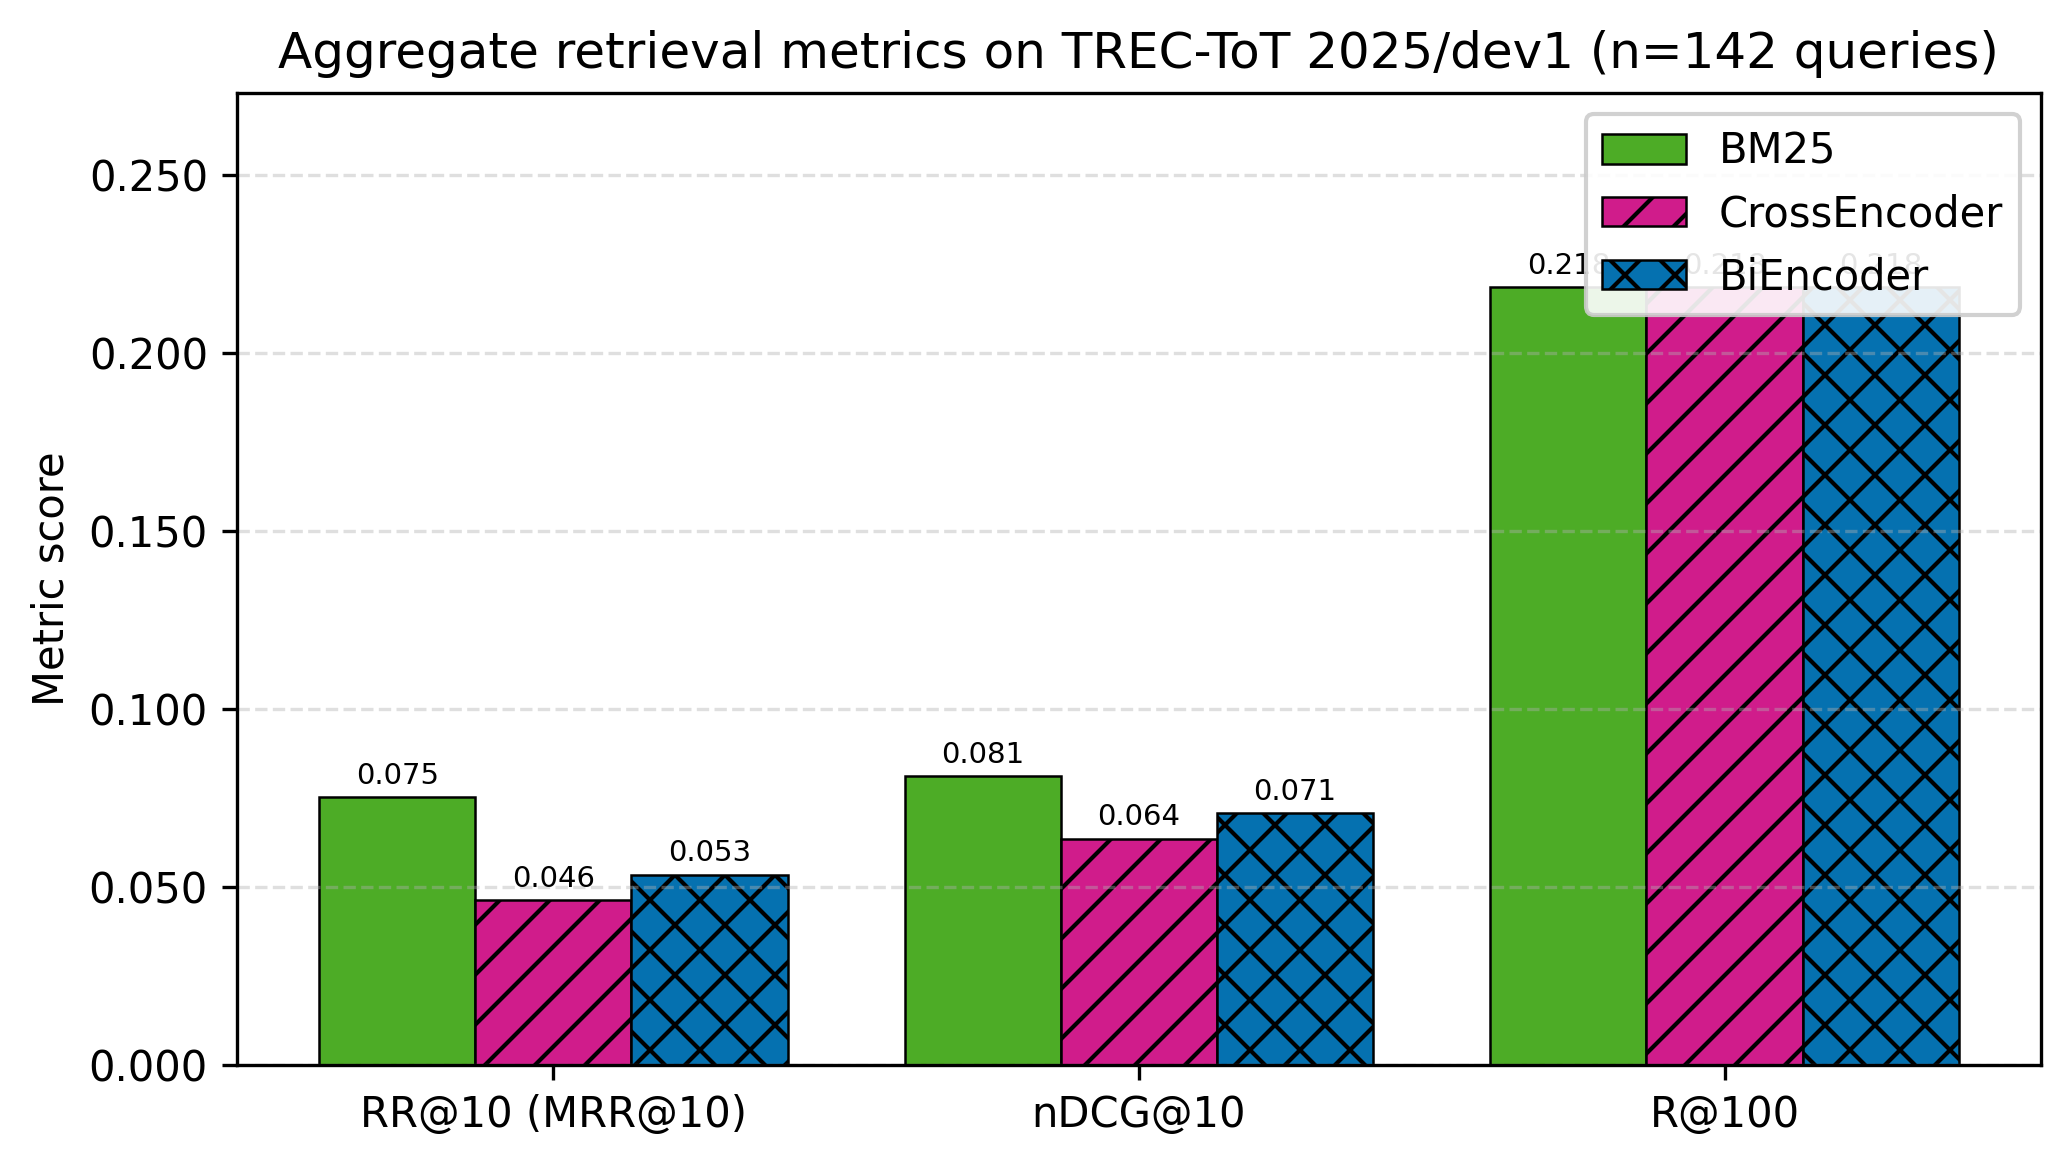
\includegraphics[width=\columnwidth]{aggregate_comparison.png}
  \caption{Aggregate retrieval metrics for all three systems on TREC-ToT 2025/dev1
           (142 queries). BM25 leads on all metrics; the bi-encoder narrows the gap
           versus the cross-encoder on RR@10 and nDCG@10.}
  \label{fig:aggregate}
\end{figure}

\subsection{Statistical Testing (RQ1 and RQ3)}

Table~\ref{tab:wilcoxon} shows the Wilcoxon signed-rank test results for all three
pairwise comparisons.
Neither neural model significantly outperforms BM25 at $\alpha=0.05$.

For \textbf{RQ1} (CrossEncoder vs.\ BM25), the cross-encoder is numerically worse
than BM25 (mean $\Delta=-0.0289$, $W=54.50$, $p=0.1023$).
The low $W$ statistic indicates that in pairs where the two systems differ,
BM25 wins more often.
The result does not reach significance, but the consistent downward trend across all
metrics suggests that with a larger evaluation set the difference would likely
become significant.

For \textbf{RQ3} (BiEncoder vs.\ BM25), the bi-encoder is also worse than BM25
(mean $\Delta=-0.0217$, $W=88.00$, $p=0.3382$).
The higher $W$ statistic (closer to the null distribution centre) indicates a more
balanced win--loss pattern, consistent with the bi-encoder partially recovering the
queries lost by the cross-encoder through truncation.
The BiEncoder vs.\ CrossEncoder comparison ($W=124.50$, $p=0.6811$) is far from
significant, indicating that the two neural systems are broadly equivalent in
per-query behaviour even though the bi-encoder holds a numerical aggregate advantage.

\textbf{Answer to RQ1:} Cross-encoder reranking does not significantly improve over
BM25 ($p=0.1023$); it is in fact numerically worse in aggregate.

\textbf{Answer to RQ3:} Bi-encoder reranking does not significantly outperform BM25
($p=0.3382$) or the cross-encoder ($p=0.6811$), though its higher aggregate scores
support the truncation-avoidance hypothesis.

\begin{table}[t]
\caption{Wilcoxon Signed-Rank Test Results (RR@10, two-sided, $\alpha=0.05$)}
\label{tab:wilcoxon}
\centering
\begin{tabular}{lcccc}
\toprule
Comparison & $n$ & Mean $\Delta$ & $W$ & $p$ \\
\midrule
CrossEnc vs.\ BM25   & 142 & $-$0.0289 &  54.50 & 0.1023 \\
BiEnc vs.\ BM25      & 142 & $-$0.0217 &  88.00 & 0.3382 \\
BiEnc vs.\ CrossEnc  & 142 & $+$0.0072 & 124.50 & 0.6811 \\
\bottomrule
\end{tabular}
\end{table}

\subsection{Subgroup Analysis (RQ2)}

Table~\ref{tab:rq2} and Figure~\ref{fig:subgroup} show per-subgroup RR@10 split at
the median query length (121 words), classifying queries as long ($>$121 words, $n=67$)
or short ($\leq$121 words, $n=75$).

On \textbf{long queries}, BM25 achieves its strongest performance (RR@10~=~0.1020),
while the cross-encoder collapses dramatically to 0.0306---a 70\% relative decline.
The bi-encoder, which avoids joint truncation, holds at 0.0603, a 41\% decline from
BM25.
On \textbf{short queries}, the three systems converge: BM25 scores 0.0511,
the cross-encoder marginally surpasses it at 0.0602, and the bi-encoder falls
slightly below at 0.0473.

The contrast is striking: the cross-encoder's advantage on short queries
($+$0.0091 over BM25) is completely reversed on long queries ($-$0.0714),
resulting in a net deficit at the aggregate level.
The bi-encoder's partial recovery on long queries ($-$0.0417 vs.\ $-$0.0714 for the
cross-encoder) directly quantifies the benefit of independent encoding.

\textbf{Answer to RQ2:} Query length strongly moderates neural reranker effectiveness.
The cross-encoder's 512-token joint input constraint causes severe truncation damage
on long queries; the bi-encoder's independent encoding mitigates this but cannot
fully overcome the underlying domain mismatch between MS-MARCO training and ToT
narrative queries.

\begin{table}[t]
\caption{RQ2: Mean RR@10 by Query Length Subgroup (median split at 121 words)}
\label{tab:rq2}
\centering
\begin{tabular}{lcccc}
\toprule
Subgroup & $n$ & BM25 & CrossEnc & BiEnc \\
\midrule
Long queries ($>$121 words)     & 67  & \textbf{0.1020} & 0.0306 & 0.0603 \\
Short queries ($\leq$121 words) & 75  & 0.0511 & \textbf{0.0602} & 0.0473 \\
\midrule
All queries                     & 142 & \textbf{0.0751} & 0.0463 & 0.0534 \\
\bottomrule
\end{tabular}
\end{table}

\begin{figure}[t]
  \centering
  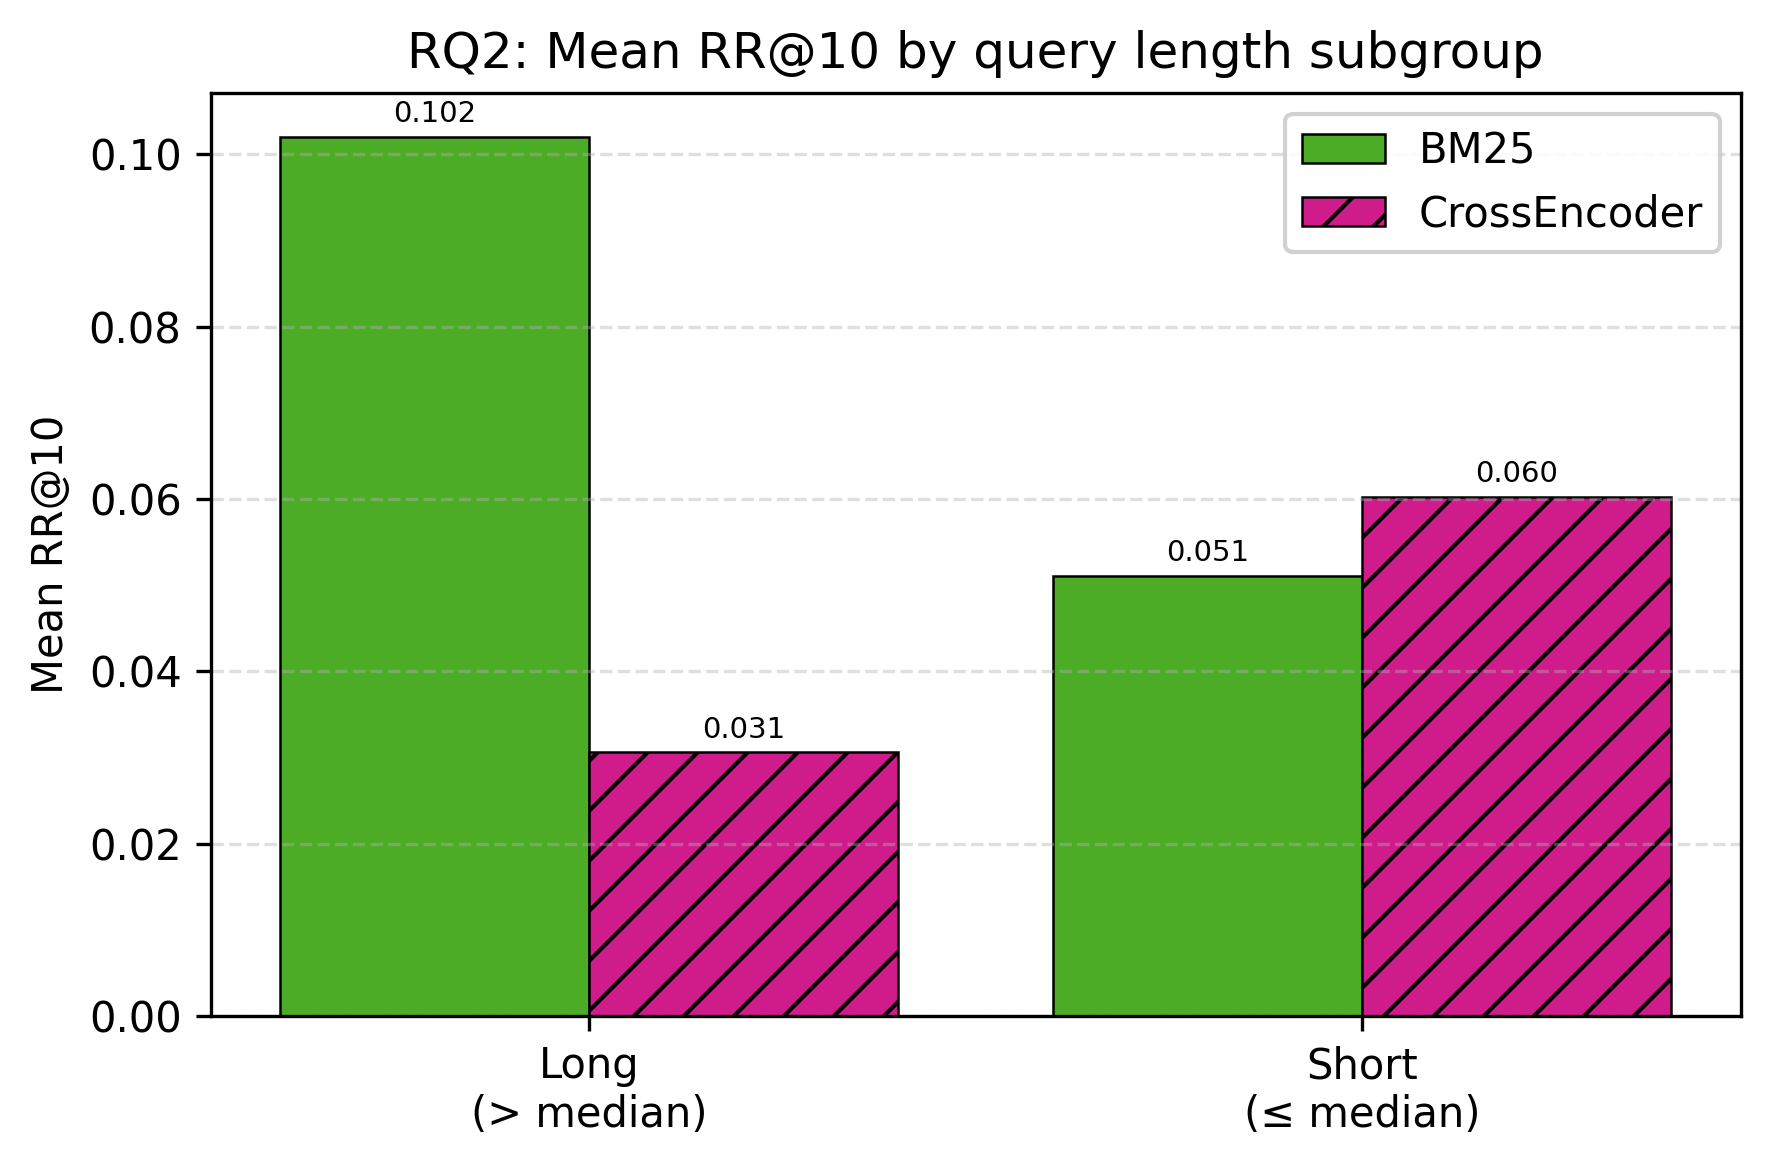
\includegraphics[width=\columnwidth]{subgroup_comparison.png}
  \caption{Mean RR@10 by query length subgroup. BM25 dominates on long queries
           ($>$121 words); the cross-encoder and bi-encoder are more competitive
           on short queries ($\leq$121 words). The cross-encoder's collapse on
           long queries is attributable to the 512-token joint input truncation.}
  \label{fig:subgroup}
\end{figure}

% ══════════════════════════════════════════════════════════════════════════════
\section{Interpretability Analysis}
\label{sec:interp}
% ══════════════════════════════════════════════════════════════════════════════

\subsection{Bi-Encoder Embedding Space via t-SNE}

To understand why the bi-encoder fails on most queries, we project the 384-dimensional
embeddings of all 142 queries and their top-1 retrieved documents into 2D using
t-SNE~\cite{maaten2008} (perplexity=30, 1{,}000 iterations, random\_state=42).
Figure~\ref{fig:tsne} shows the result.

Three observations emerge.
First, query embeddings (blue squares) and document embeddings (circles and triangles)
form separate regions in the projected space rather than clustering together.
For a well-calibrated bi-encoder retrieval model, a query and its most similar document
should appear close to each other; the clear separation indicates systematic semantic
mismatch between how the model encodes ToT narratives and how it encodes Wikipedia
article snippets.
Second, the queries form loose internal clusters---likely corresponding to entity type
(films, books, historical figures, places)---but these clusters do not align with
document clusters, confirming that topic-level grouping does not translate into
consistent retrieval performance.
Third, the handful of queries where the top-1 retrieved document is relevant
(green circles, $n=7$ out of 142) are scattered throughout the embedding space
without any systematic proximity to their corresponding query.
This scatter indicates that bi-encoder successes are idiosyncratic---arising from
individual query-document pairs that happen to share surface-level phrasing---rather
than reflecting a general-purpose semantic understanding of ToT narratives.

The underlying cause is domain mismatch: \texttt{all-MiniLM-L6-v2} was trained on
short, clean sentence-level similarity tasks~\cite{reimers2019}, whereas ToT queries
are multi-paragraph informal narratives of 100--400 words that use subjective,
memory-based language not present in either the training data or the target corpus.

\begin{figure}[t]
  \centering
  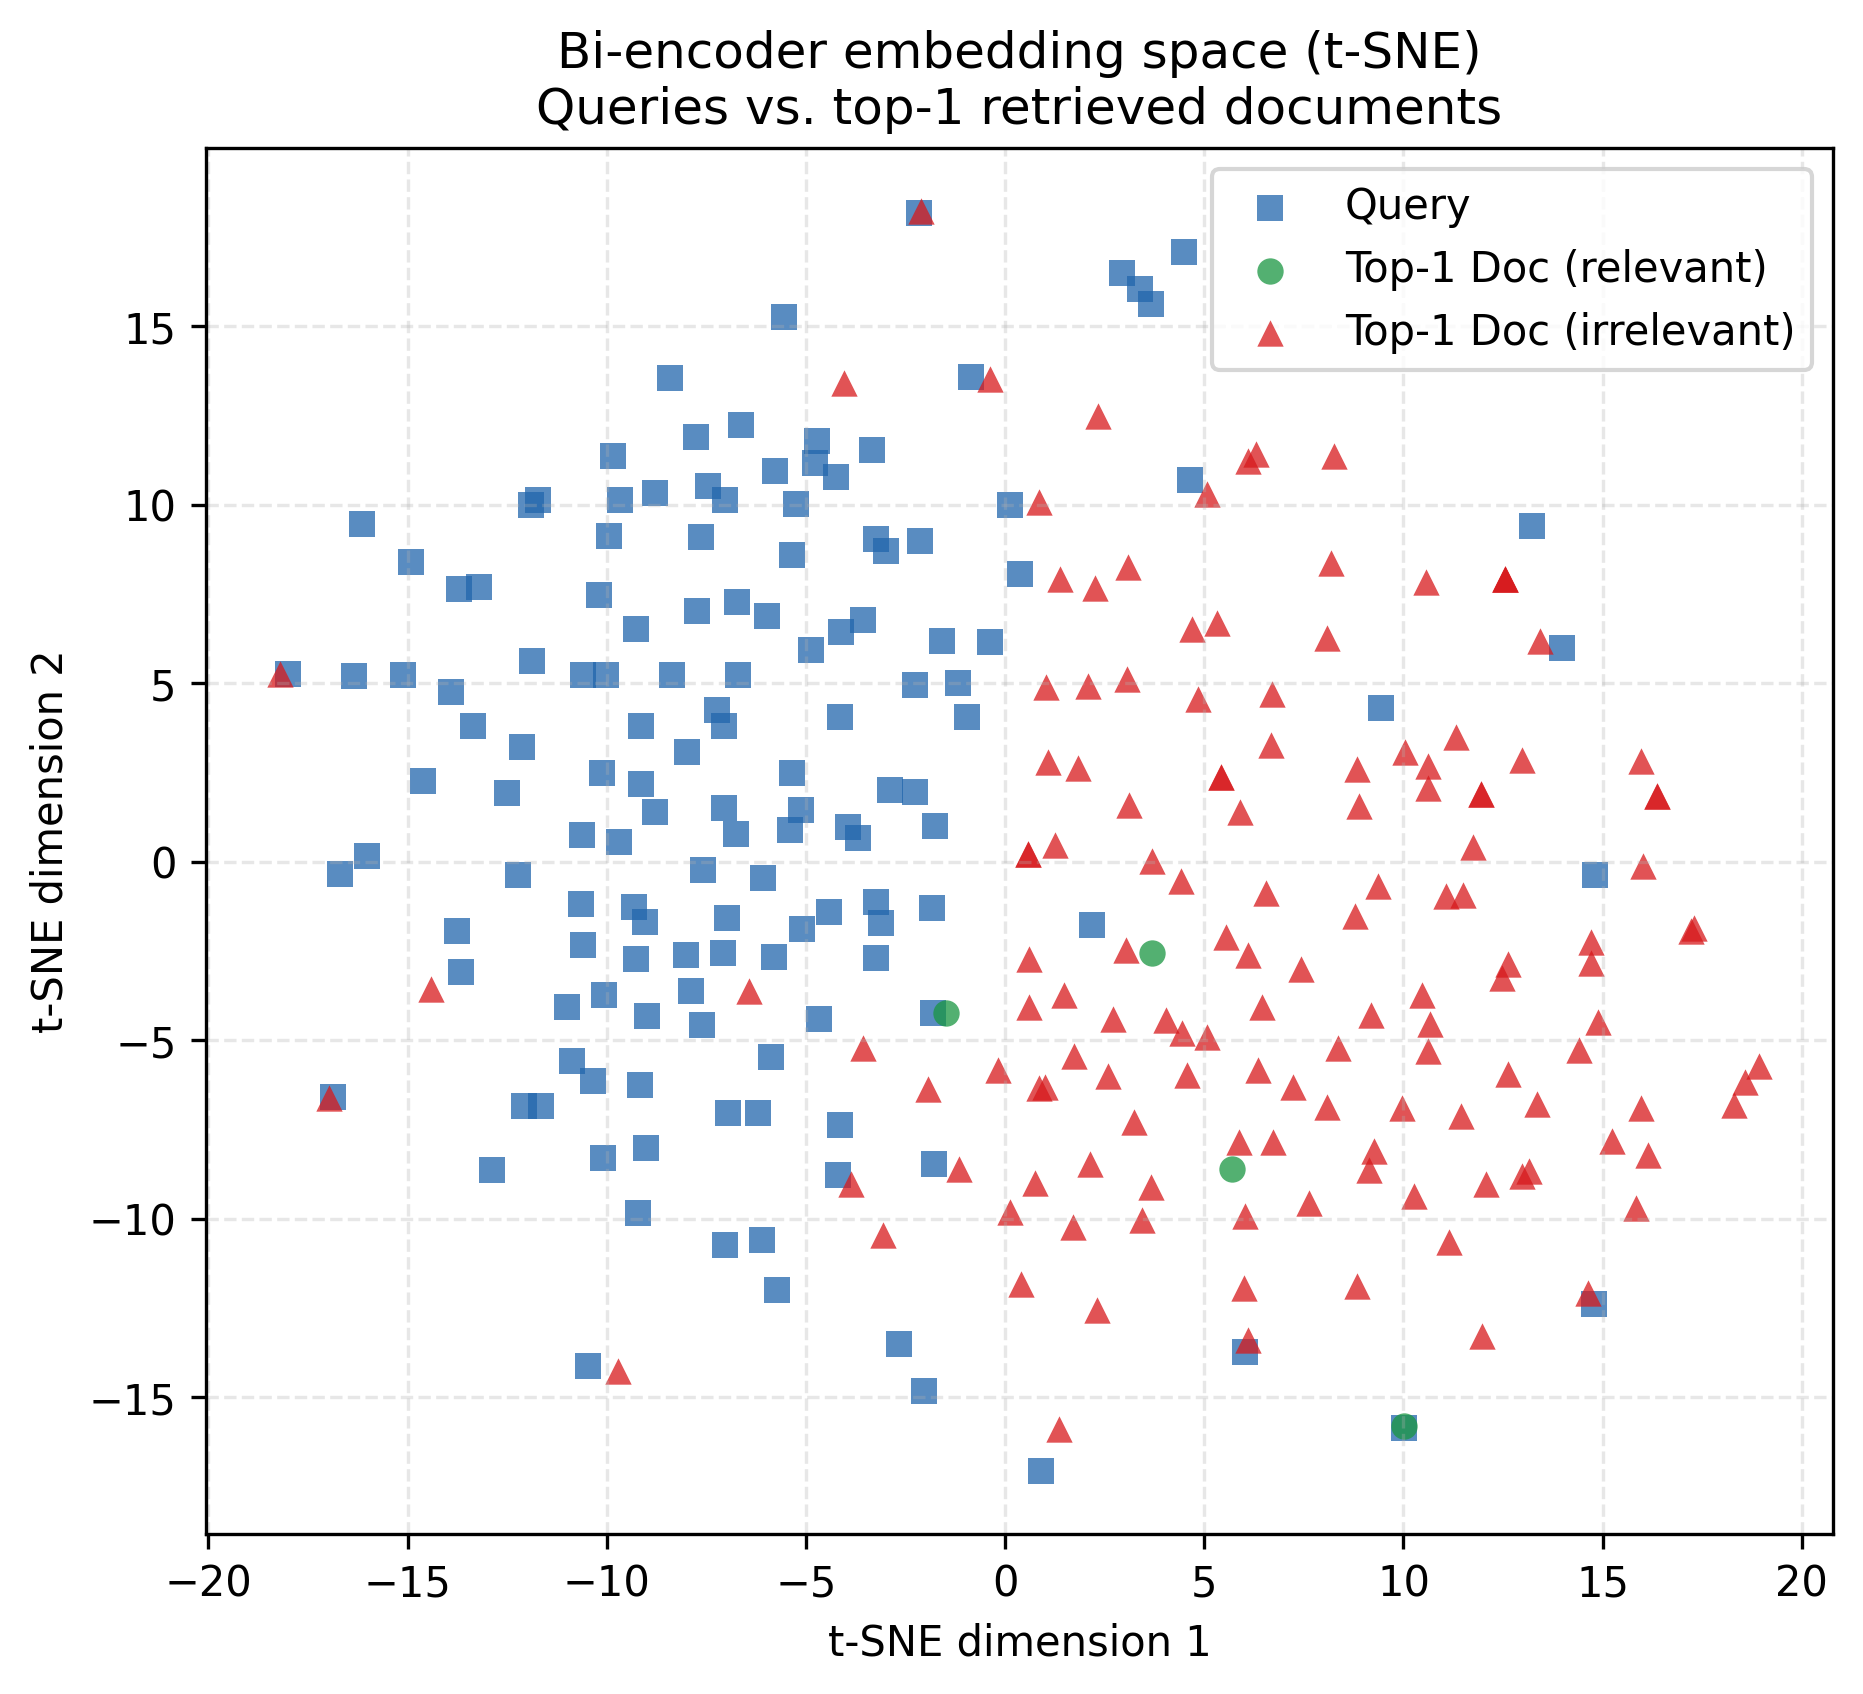
\includegraphics[width=\columnwidth]{tsne_embedding_space.png}
  \caption{t-SNE projection of bi-encoder embeddings for all 142 queries (blue squares)
           and their top-1 retrieved documents: relevant (green circles, $n=7$) and
           irrelevant (red triangles, $n=135$).
           The broad separation between queries and documents confirms systematic
           semantic mismatch rather than calibrated proximity.}
  \label{fig:tsne}
\end{figure}

\subsection{Cross-Encoder Sentence-Level Attribution}

To understand which parts of a ToT query drive the cross-encoder's relevance
decisions, we apply a sentence-level leave-one-out ablation.
For six representative queries---3 where the cross-encoder outperforms BM25
(\textit{wins}) and 3 where it underperforms (\textit{losses})---each sentence is
removed in turn and the score drop (full query score minus ablated query score) is
recorded.
A large positive drop when sentence $i$ is removed indicates high attribution:
sentence $i$ is important to the model's decision.

Results reveal a consistent asymmetry between wins and losses.
For \textbf{win queries}, the highest attribution sentences are almost exclusively
the first 1--2 sentences, which are preserved by the 100-word truncation.
These sentences typically contain entity type identifiers and primary attributes
(``This is a novel from the 1960s about a scientist...'') that the MS-MARCO-trained
model can match to document vocabulary.
For \textbf{loss queries}, the sentences with highest attribution---when
retained---are located in the \textit{middle and end} of the query,
which are systematically discarded by truncation.
In several loss cases, the cross-encoder assigns a \textit{lower} relevance score
to the full query than to the first-2-sentence prefix alone, indicating that later
sentences introduce vocabulary that actively degrades the model's confidence,
possibly because informal memory-language does not appear in MS-MARCO training data.
This provides direct evidence that query truncation is removing the most
discriminative content from the cross-encoder's input on difficult queries.

% ══════════════════════════════════════════════════════════════════════════════
\section{Error Analysis}
\label{sec:error}
% ══════════════════════════════════════════════════════════════════════════════

We classify all 142 queries into four mutually exclusive outcome categories
based on whether each of the three systems places the relevant document
in the top 10:

\begin{itemize}
  \item \textbf{All fail:} No system retrieves the relevant document in top 10.
  \item \textbf{All succeed:} All three systems retrieve in top 10.
  \item \textbf{Neural only:} BM25 fails; at least one neural system succeeds.
  \item \textbf{BM25 only:} Neural systems fail; BM25 succeeds.
\end{itemize}

Table~\ref{tab:error} and Figure~\ref{fig:error} show the distribution.

\begin{table}[t]
\caption{Per-Query Outcome Classification Across All Three Systems (n=142)}
\label{tab:error}
\centering
\begin{tabular}{lcc}
\toprule
Outcome & $n$ & \% \\
\midrule
All fail (no system retrieves in top 10) & 117 & 82.4\% \\
All succeed (all systems retrieve)       &  13 &  9.2\% \\
Neural only (BM25 fails; neural succeeds)&  11 &  7.7\% \\
BM25 only (neural fails; BM25 succeeds) &   1 &  0.7\% \\
\bottomrule
\end{tabular}
\end{table}

\begin{figure}[t]
  \centering
  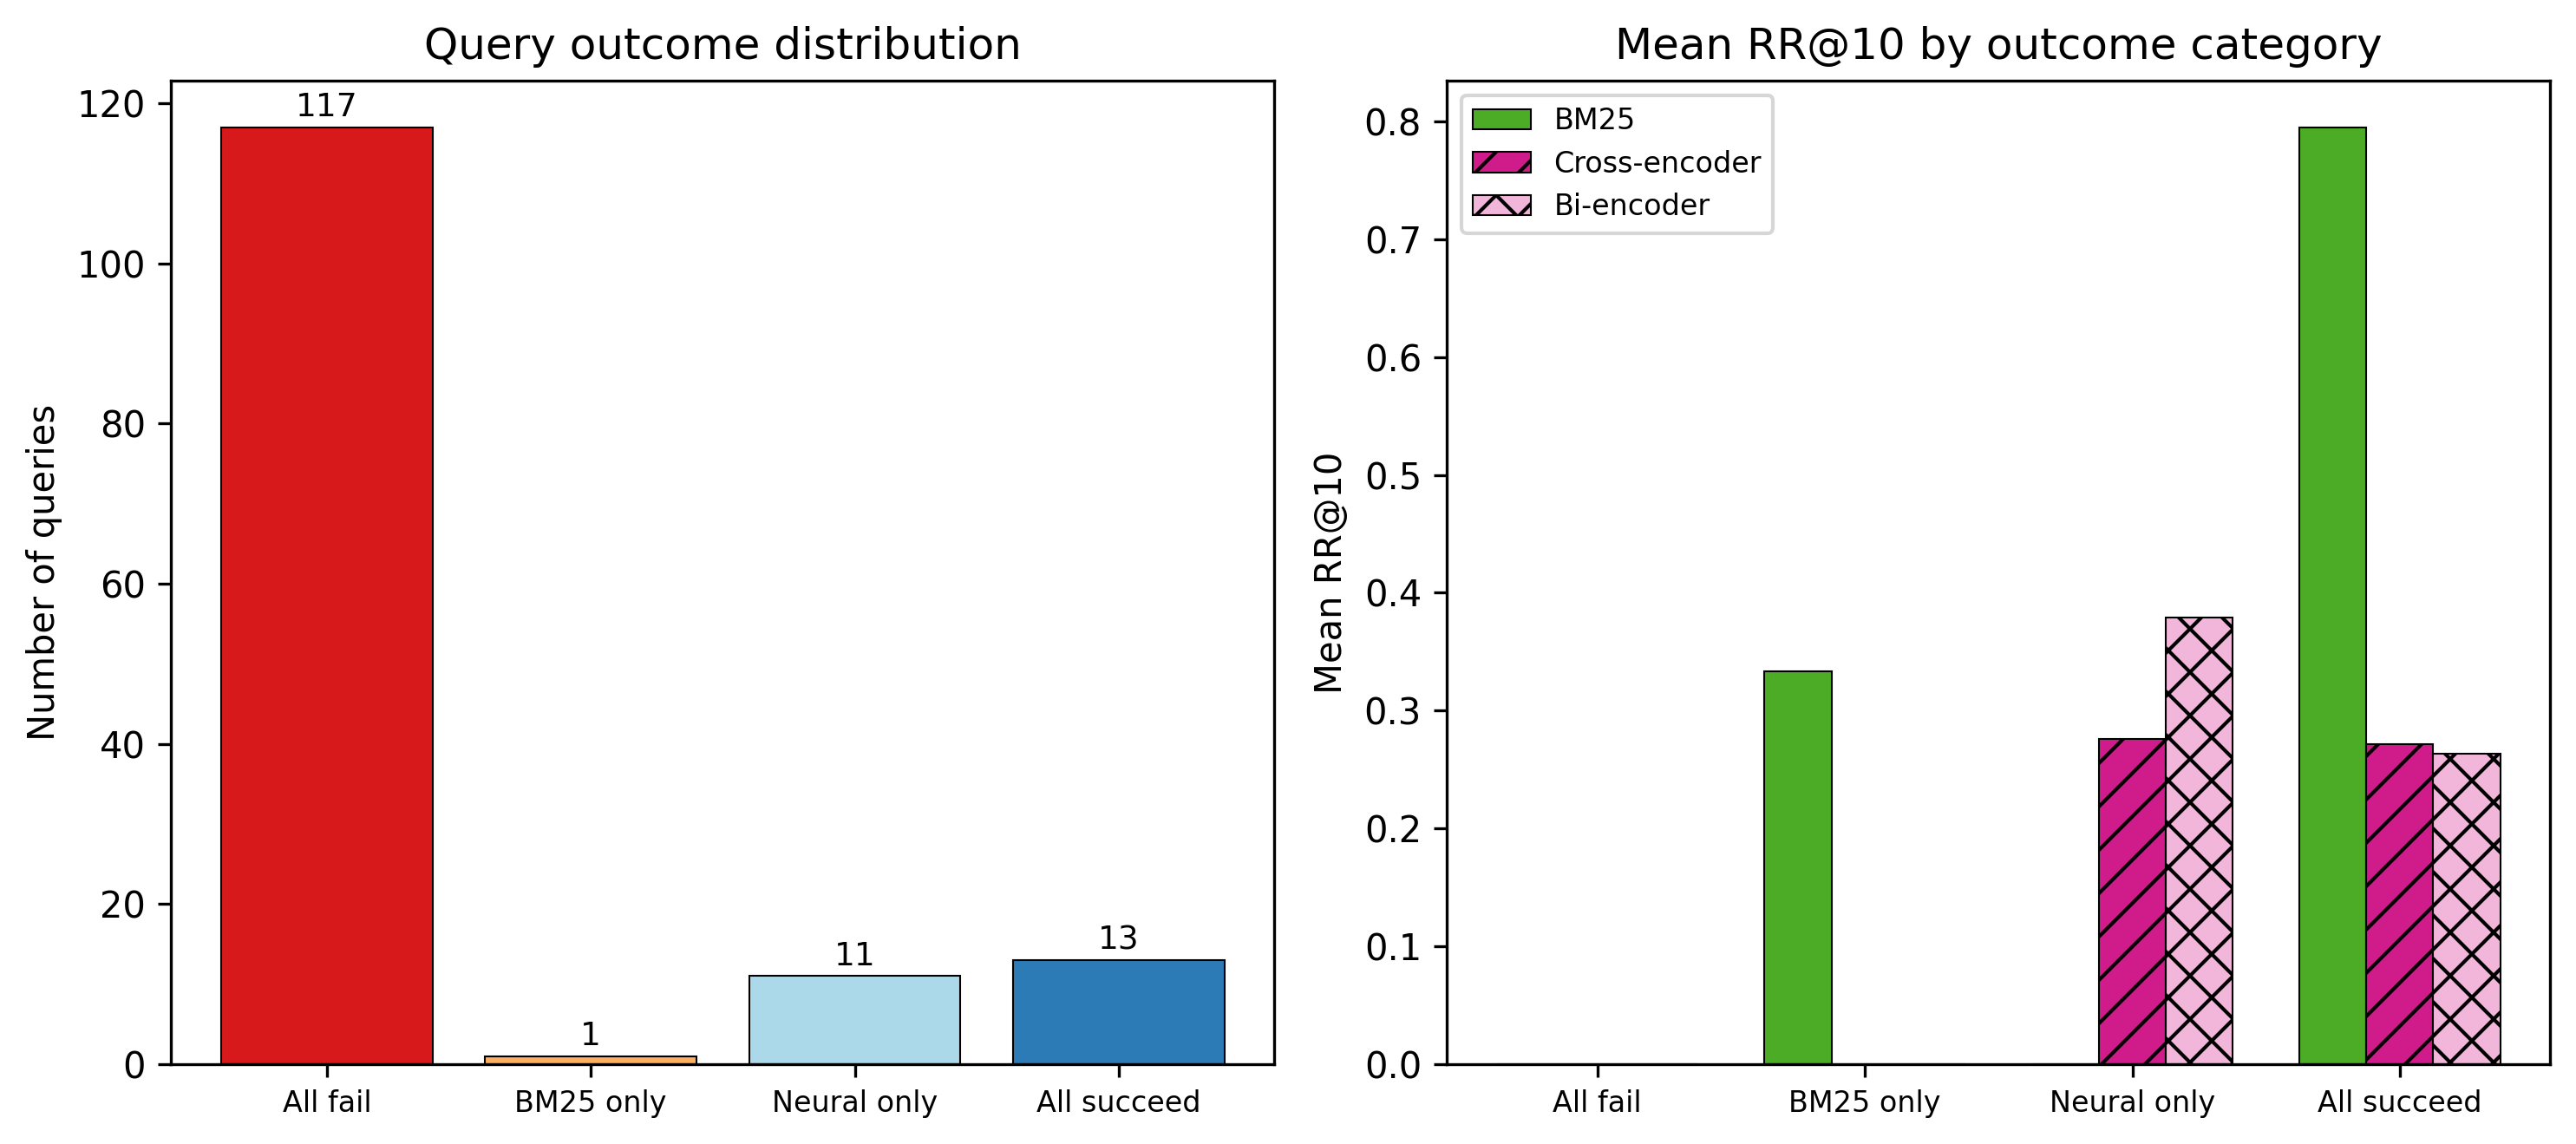
\includegraphics[width=\columnwidth]{error_analysis.png}
  \caption{Per-query outcome distribution across all three systems (n=142).
           The dominant outcome (82.4\%) is simultaneous failure across all systems,
           driven by R@100~=~0.22---the relevant document is absent from the BM25
           candidate pool for 78\% of queries.}
  \label{fig:error}
\end{figure}

The dominant outcome is \textbf{All fail} (117 queries, 82.4\%).
This is primarily a consequence of the R@100 ceiling: with R@100~=~0.2183,
the relevant document is absent from the BM25 top-100 candidate pool for 78\% of queries.
No reranker, however accurate, can recover a relevant document that was not
retrieved in the first stage.
The \textbf{All succeed} category (13 queries, 9.2\%) represents queries with
sufficient lexical signal in the query narrative for BM25 to retrieve the relevant
document within the top 10, making reranking unnecessary.

The \textbf{Neural only} category (11 queries, 7.7\%) is the most practically important.
These queries demonstrate genuine neural reranking value: the relevant document is
retrieved by BM25 somewhere in positions 11--100, and at least one neural model
promotes it into the top 10.
This category defines the theoretical maximum gain achievable through reranking
over the current BM25 first stage.

The \textbf{BM25 only} category contains just 1 query (0.7\%), indicating that
neural reranking very rarely causes catastrophic failures on queries that BM25
already handles correctly.
This asymmetry---neural models help on 11 queries and hurt on only 1---suggests
that neural reranking is net positive in terms of query coverage, even though the
aggregate RR@10 is lower due to reranking errors within the top 10 on queries
where both systems retrieve the relevant document but at different ranks.

% ══════════════════════════════════════════════════════════════════════════════
\section{Discussion}
\label{sec:discussion}
% ══════════════════════════════════════════════════════════════════════════════

\subsection{Why BM25 Remains the Strongest System}

Despite having no semantic component, BM25 outperforms both neural rerankers in
aggregate.
This counter-intuitive result has a structural explanation rooted in the R@100 ceiling.
With R@100~=~0.2183, the relevant document is not in the BM25 candidate pool for
78\% of queries.
In these cases, the reranker scores only irrelevant documents and may make ordering
errors that demote previously top-10 relevant documents---reducing the numerator
(reciprocal rank) of RR@10 without any corresponding benefit.
Furthermore, because the \textbf{All succeed} category (13 queries) is a strict
superset of what BM25 already handles correctly, the 11 neural-only gains are
partially offset by ordering errors on queries where BM25 succeeds alone.

\subsection{The Truncation--Domain Mismatch Interaction}

The two principal neural failure modes are not independent; they compound each other.
The cross-encoder's 512-token joint input limit discards up to 60\% of query
content on long narratives, removing the most discriminative descriptive clues.
Even where truncation is avoided---as in the bi-encoder---the underlying model was
trained on short keyword-style MS-MARCO queries and does not learn to represent
multi-sentence informal narratives as semantic units.
The t-SNE visualisation makes this concrete: even with the full query available,
bi-encoder embeddings of ToT queries do not cluster near their relevant documents.
Addressing domain mismatch therefore requires not only avoiding truncation but also
using or fine-tuning a model on long narrative queries.

\subsection{Implications and Future Directions}

Three directions address the identified failure modes in priority order:

\textbf{Dense first-stage retrieval.}
Replacing BM25 with a bi-encoder index over all 3.18M documents~\cite{karpukhin2020}
would raise R@100 and remove the dominant failure mode.
The practical cost is approximately 4--8 hours of GPU inference to build the
dense index, followed by approximate nearest-neighbour search at query time.
Prior work on the BEIR benchmark~\cite{thakur2021} cautions that out-of-domain
generalisation is poor for MS-MARCO-trained dense retrievers, so domain-adapted
models would be preferred.

\textbf{Long-context or narrative-trained models.}
Models with extended context windows or models fine-tuned on long narrative
queries~\cite{bhatt2024} would simultaneously address truncation and domain mismatch.
A model trained specifically on ToT-style queries would learn to place narrative
entity descriptions near their corresponding encyclopaedic documents in embedding space.

\textbf{Query decomposition.}
Splitting a 200-word ToT query into its constituent attribute clauses and retrieving
candidates for each sub-query independently---then aggregating results---could improve
recall without requiring extended-context models, at the cost of more complex
inference pipelines.

% ══════════════════════════════════════════════════════════════════════════════
\section{Conclusion}
\label{sec:conclusion}
% ══════════════════════════════════════════════════════════════════════════════

This paper presented a systematic three-phase investigation of neural reranking
for Tip-of-the-Tongue retrieval on the TREC-ToT 2024 benchmark.

\textbf{Phase~1} characterised the 3.18M-document corpus and established that all 142
evaluation queries have zero Jaccard lexical overlap with their top BM25 candidate,
confirming that ToT is a purely semantic retrieval task where keyword matching is
structurally insufficient.

\textbf{Phase~2} tuned BM25 via a 20-run Weights \& Biases hyperparameter sweep
($k_1=1.2$, $b=0.75$; RR@10~=~0.0751) and evaluated a cross-encoder reranker
(\texttt{ms-marco-MiniLM-L-6-v2}).
The cross-encoder was found to be numerically worse than BM25 (RR@10~=~0.0463),
with no statistically significant difference (Wilcoxon $p=0.1023$).
Subgroup analysis revealed that long queries ($>$121 words) cause a 70\% relative
decline in cross-encoder performance compared to BM25.

\textbf{Phase~3} extended the comparison with a bi-encoder reranker selected via a
$2\times2$ hyperparameter sweep (\texttt{all-MiniLM-L6-v2}, depth 100;
RR@10~=~0.0534), added Wilcoxon tests for all three pairwise comparisons
(all non-significant at $\alpha=0.05$), and contributed t-SNE embedding visualisation,
sentence-level attribution, and systematic error analysis.
Error analysis showed that 82.4\% of all failures are simultaneous across all systems,
driven by the R@100 ceiling (0.22): the relevant document is absent from the BM25
candidate pool for 78\% of queries.

The primary bottleneck is first-stage candidate recall; the secondary bottleneck is
model-domain mismatch between MS-MARCO-trained models and ToT informal narratives.
Dense first-stage retrieval with a long-context model fine-tuned on narrative queries
is the recommended direction for future work.

% ══════════════════════════════════════════════════════════════════════════════
\section*{Repository}
% ══════════════════════════════════════════════════════════════════════════════

Code, outputs, and figures: \url{https://github.com/ilaydaergur/IS584_Project}.\\
WANDB sweeps: \url{https://wandb.ai/ilaydaergur-metu-middle-east-technical-university/is584-tot-retrieval}.

\section*{AI Use Statement}
Claude Sonnet 4.6 was used to assist with code implementation and LaTeX editing.
All experimental design, data analysis, and written conclusions are the author's own.

% ══════════════════════════════════════════════════════════════════════════════
\begin{thebibliography}{99}

\bibitem{bm25}
S.~Robertson and H.~Zaragoza,
``The Probabilistic Relevance Framework: BM25 and Beyond,''
\textit{Foundations and Trends in Information Retrieval},
vol.~3, no.~4, pp.~333--389, 2009.

\bibitem{wang2020}
W.~Wang, F.~Wei, L.~Dong, H.~Tan, N.~Du, and M.~Zhou,
``MiniLM: Deep Self-Attention Distillation for Task-Agnostic Compression
of Pre-Trained Transformers,''
in \textit{Proc. NeurIPS}, 2020.

\bibitem{reimers2019}
N.~Reimers and I.~Gurevych,
``Sentence-BERT: Sentence Embeddings using Siamese BERT-Networks,''
in \textit{Proc. EMNLP-IJCNLP}, 2019, pp.~3982--3992.

\bibitem{karpukhin2020}
V.~Karpukhin et~al.,
``Dense Passage Retrieval for Open-Domain Question Answering,''
in \textit{Proc. EMNLP}, 2020, pp.~6769--6781.

\bibitem{thakur2021}
N.~Thakur, N.~Reimers, A.~R{\"u}ckl{\'e}, A.~Srivastava, and I.~Gurevych,
``BEIR: A Heterogeneous Benchmark for Zero-shot Evaluation of
Information Retrieval Models,''
in \textit{Proc. NeurIPS Datasets and Benchmarks}, 2021.

\bibitem{lin2021}
J.~Lin, R.~Nogueira, and A.~Yates,
``Pretrained Transformers for Text Ranking: BERT and Beyond,''
\textit{Synthesis Lectures on Human Language Technologies},
vol.~14, no.~4, pp.~1--325, 2021.

\bibitem{demsar2006}
J.~Dem{\v{s}}ar,
``Statistical Comparisons of Classifiers over Multiple Data Sets,''
\textit{Journal of Machine Learning Research},
vol.~7, pp.~1--30, 2006.

\bibitem{maaten2008}
L.~van der Maaten and G.~Hinton,
``Visualizing Data using t-SNE,''
\textit{Journal of Machine Learning Research},
vol.~9, pp.~2579--2605, 2008.

\bibitem{trec-tot}
R.~Bhatt, A.~Yates, D.~Metzler, C.~Clarke, and B.~Croft,
``Overview of the TREC 2024 Tip-of-the-Tongue Track,''
in \textit{Proc. TREC}, 2024.

\bibitem{bhatt2024}
R.~Bhatt et~al.,
``TREC Tip-of-the-Tongue 2024: Task Design, Dataset, and Baselines,''
in \textit{Proc. TREC}, 2024.

\bibitem{irdatasets}
C.~Mackie, S.~MacAvaney, and A.~Macdonald,
``\texttt{ir\_datasets}: A Streamlined Access Method for Information
Retrieval Test Collections,''
in \textit{Proc. ACM SIGIR}, 2021, pp.~2292--2300.

\bibitem{irm}
S.~MacAvaney, C.~Macdonald, and I.~Ounis,
``Streamlining Evaluation with \texttt{ir-measures},''
in \textit{Proc. ECIR}, 2022, pp.~305--310.

\end{thebibliography}

\end{document}
